\documentclass{beamer}

% For more themes, color themes and font themes, see:
% http://deic.uab.es/~iblanes/beamer_gallery/index_by_theme.html
%
\mode<presentation>
{
  \usetheme{Madrid}       % or try default, Darmstadt, Warsaw, ...
  \usecolortheme{crane} % or try albatross, beaver, crane, ...
  \usefonttheme{serif}    % or try default, structurebold, ...
  \setbeamertemplate{navigation symbols}{}
  \setbeamertemplate{caption}[numbered]
} 

\usepackage{tikz}
\usetikzlibrary{decorations.markings,angles}
\usepackage{tikz-3dplot} 

\usepackage{amsmath}


\begin{document}



\begin{frame}{FIRS FOV}

 
\begin{figure}[H]
 \centering
 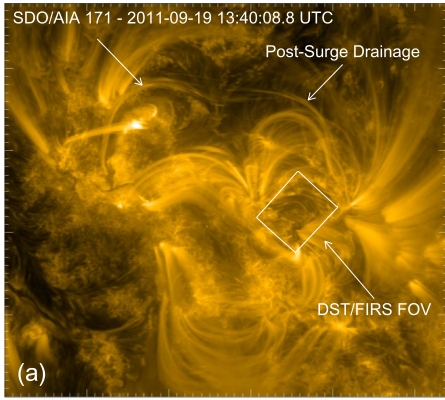
\includegraphics[scale=0.5]{img1.png}
%\caption{iron emission line at 600000K: upper transition region , quiet corona}
\end{figure}



\end{frame}

\begin{frame}{FIRS FOV}

 
\begin{figure}[H]
 \centering
 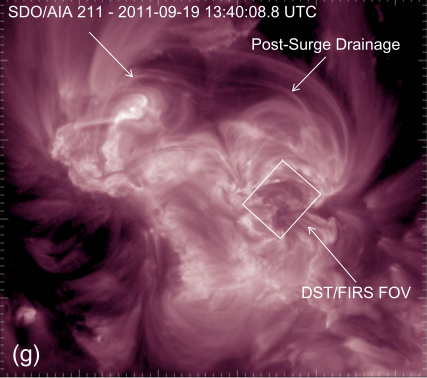
\includegraphics[scale=0.5]{img2.png}
%\caption{iron emission line at 2000000K: active regions conrona}
\end{figure}



\end{frame}

\begin{frame}{FIRS data}
\begin{itemize}
\item field of view of 60x70 arcsec
\item spatial sampling of 0.29 arcsec and an observed
spectral range of 35.743 $\AA (\Delta \lambda = 8.683 m\AA / pixel )$ 
\item the slit
was oriented at a 41.3 deg. angle with respect to the solar meridian
\item the slit was scanned from solar
northeast to southwest with a step size equal to the projected
slit width of 0 29. 
\item At each slit position, spectra were acquired
using a sequence of four efficiency-balanced modulation states
using 125 ms exposures, which was repeated once for a total of
1 s cumulative integration time. The 218 step scan lasted
32 minutes

\end{itemize}
\end{frame}


\begin{frame}{FIRS data}

time of slit scan: 16:29 - 17:01

\begin{figure}[H]
  \centering
  \begin{minipage}[b]{0.4\textwidth}
    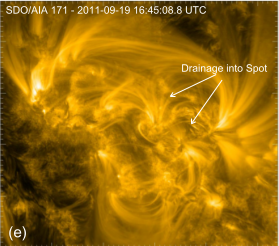
\includegraphics[scale=0.5]{img3.png}
  \end{minipage}
  \hfill
  \begin{minipage}[b]{0.4\textwidth}
    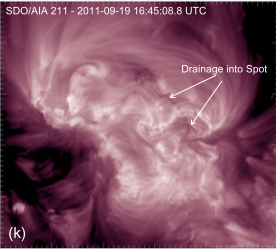
\includegraphics[scale=0.5]{img4.png}
  \end{minipage}
\end{figure}

 



\end{frame}



\begin{frame}{FIRS data}

Standard reduction methods were applied to the FIRS data in
the manner described by Schad et al. (2013), which includes
dark and flat calibrations, geometric registration, wavelength
calibration, and polarimetric cross-talk removal. One exception
here is that the spectral dispersion was determined by fitting the
line cores of the two telluric lines at 10833.981 and
10832.108 \AA , as in Kuckein et al. (2012b). Residual inter-
ference fringes were removed from the polarized spectra using
the 2D pattern recognition technique of Casini et al. (2012),
resulting in an unbinned mean noise level in Stokes (Q, U, V)
of (1.0, 0.92, 1.3)$10^{-3}$ , in units of the incident intensity.
The reference direction for Stokes+Q is parallel to the solar
equator.

Despite real-time seeing correction and image stabilization
by the DST high-order adaptive optics system (Rimmele
et al. 2004), the solar image experienced shifts up to 0 1
between adjacent FIRS slit positions due to short periods of
degraded atmospheric seeing, with a cumulative temporal drift
of 2 55 during the scan. These shifts have been corrected
through careful image registration with a co-operating G-band
context imager. Image shifts determined from the G-band
images are converted to their equivalent shift within the FIRS
map. Any spatial maps of feature topology or physical
quantities derived from the FIRS maps are corrected using
Delaunay triangulation of the translated observation points
(Lee, Schachter 1980) and subsequent quintic-polynomial
smooth interpolation

\end{frame}






\begin{frame}{He velocity along loop}

 
\begin{figure}[H]
 \centering
 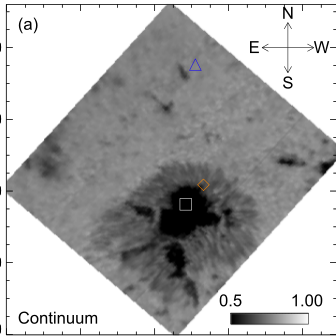
\includegraphics[scale=0.6]{sp_cont.png}
\end{figure}



\end{frame}





\begin{frame}{He velocity along loop}
 
\begin{figure}[H]
 \centering
 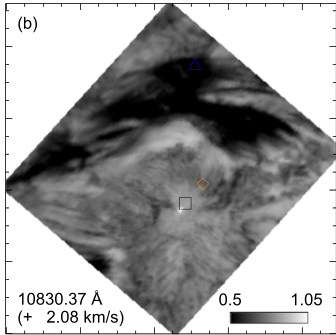
\includegraphics[scale=0.6]{spb.png}
\end{figure}

\end{frame}

\begin{frame}{He velocity along loop}
 
\begin{figure}[H]
 \centering
 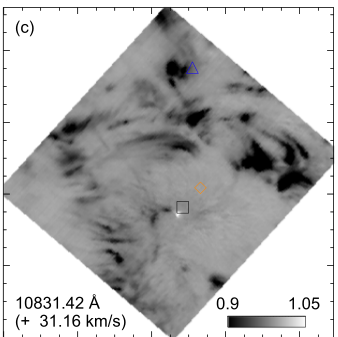
\includegraphics[scale=0.6]{spc.png}
\end{figure}

\end{frame}



\begin{frame}{He velocity along loop}
 
\begin{figure}[H]
 \centering
 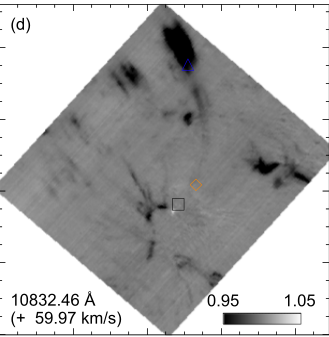
\includegraphics[scale=0.6]{spd.png}
\end{figure}

\end{frame}


\begin{frame}{He velocity along loop}
 
\begin{figure}[H]
 \centering
 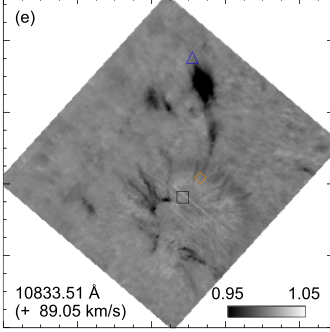
\includegraphics[scale=0.6]{spe.png}
\end{figure}

\end{frame}

\begin{frame}{He velocity along loop}
 
\begin{figure}[H]
 \centering
 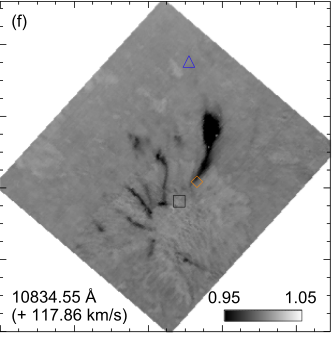
\includegraphics[scale=0.6]{spf.png}
\end{figure}

\end{frame}
\begin{frame}{He velocity along loop}
 
\begin{figure}[H]
 \centering
 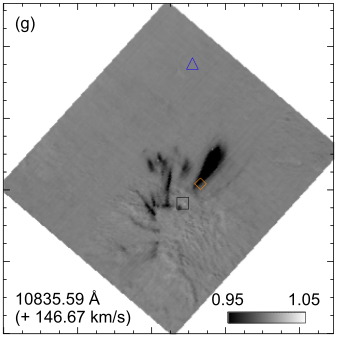
\includegraphics[scale=0.6]{spg.png}
\end{figure}

\end{frame}
\begin{frame}{He velocity along loop}
 
\begin{figure}[H]
 \centering
 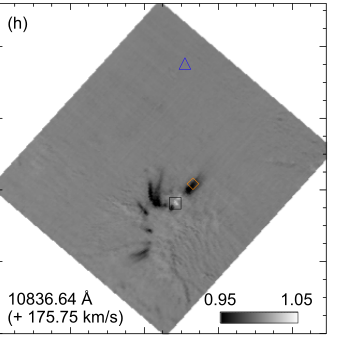
\includegraphics[scale=0.6]{sph.png}
\end{figure}

\end{frame}



\begin{frame}{He velocity along loop}

normalized to the local continuum intensity
 
\begin{figure}[H]
 \centering
 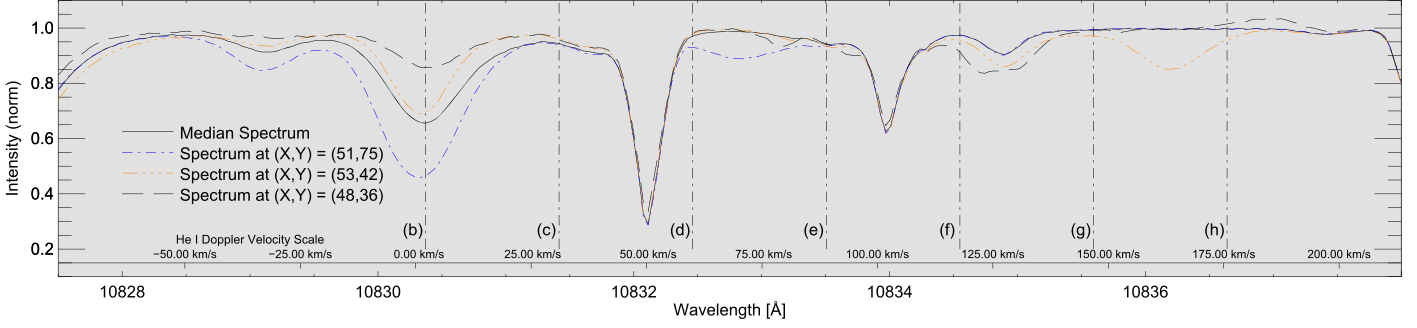
\includegraphics[scale=0.25]{sp_spec.png}
\caption{
spectral line profiles extracted from the
locations indicated in panels (a)–(h), illustrating the presence of additional He I velocity components redward of the telluric feature at 10832.1  \AA, and relative to the
median spectrum calculated using the entire data cube. An He I Doppler velocity scale bar is added for reference
}
\end{figure}



\end{frame}

\begin{frame}{Stereoscopic observations}

\begin{figure}[H]
 \centering
 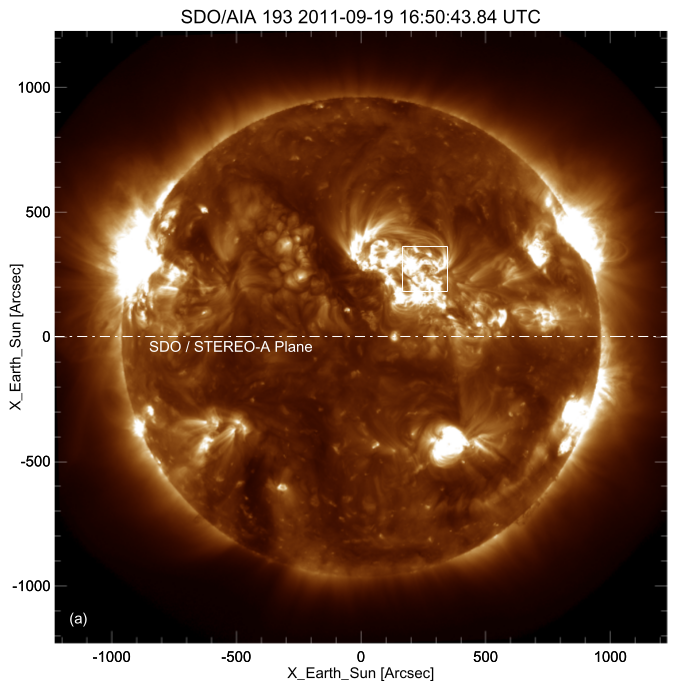
\includegraphics[scale=0.4]{sp_aia.png}
\end{figure}

\end{frame}
\begin{frame}{Stereoscopic observations}

\begin{figure}[H]
 \centering
 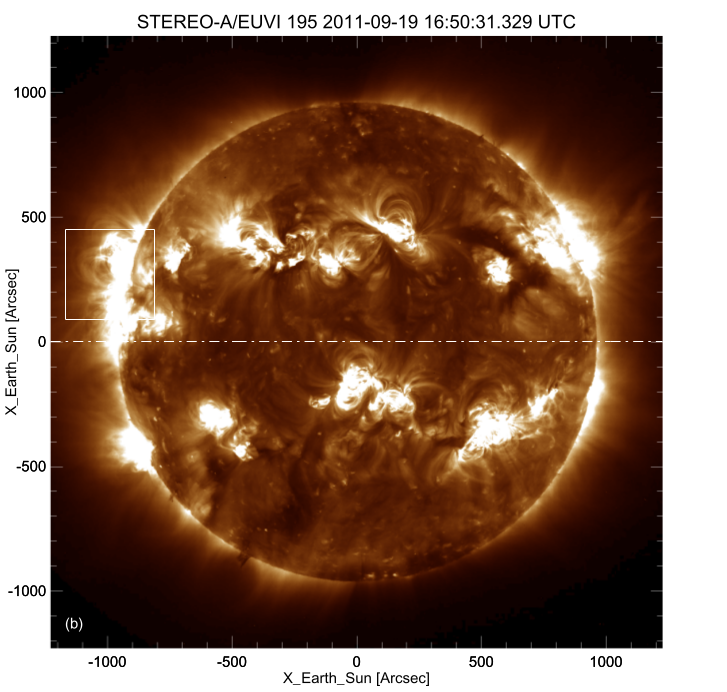
\includegraphics[scale=0.4]{sp_stereo.png}
\end{figure}

\end{frame}
\end{document}
